\documentclass[12pt]{article}
\usepackage[spanish, es-tabla]{babel}
%\usepackage[top=2.5cm, bottom=2.5cm,left=2cm, right=2cm]{geometry}
\usepackage[top=1.78cm, bottom=1.78cm,left=1.65cm, right=1.65cm]{geometry}
\usepackage[utf8x]{inputenc}
\usepackage{amsmath}
\usepackage{graphicx}
\setlength{\parindent}{12pt}
\usepackage[colorinlistoftodos]{todonotes}
\usepackage{multicol}
\let\olditemize\itemize
\def\itemize{\olditemize\itemsep=0pt }
\usepackage[hidelinks]{hyperref}

\usepackage[pages=some]{background}
\backgroundsetup{
 scale=1,
 color=black,
 opacity=0.4,
 angle=0,
 contents={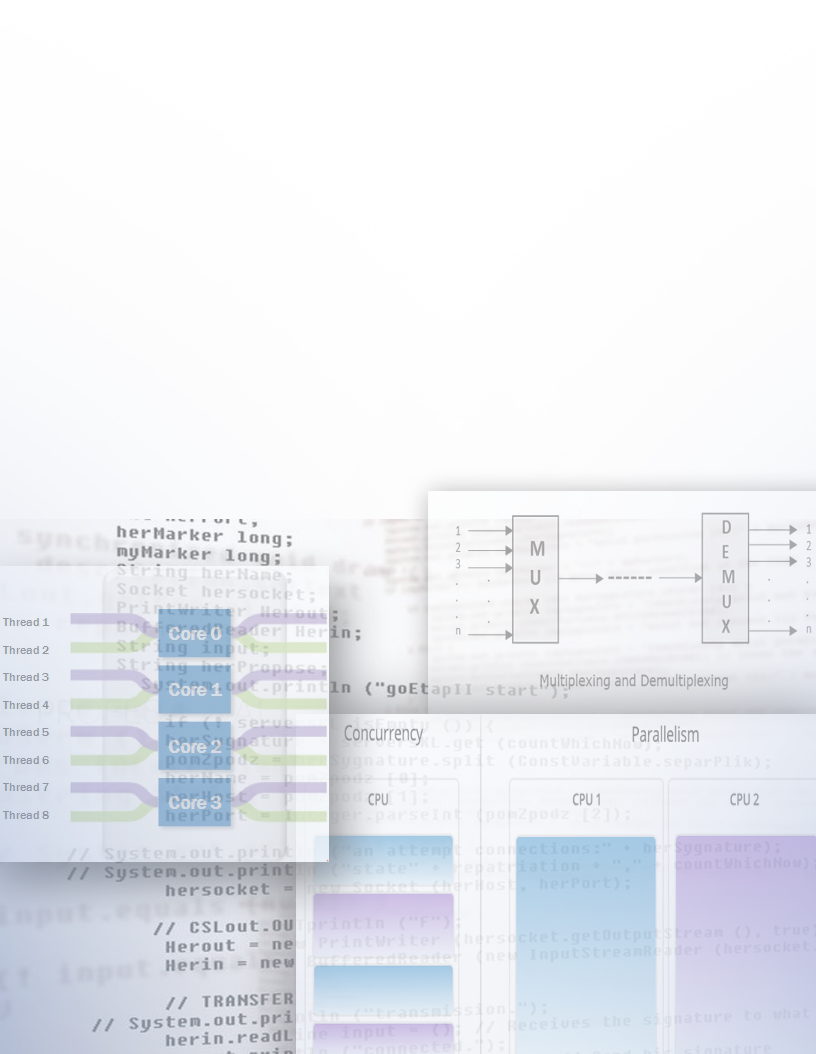
\includegraphics[scale=0.7]{BG.png}
 }
}

\begin{document}
\begin{titlepage}
\BgThispage
\newcommand{\HRule}{\rule{\linewidth}{0.5mm}}
\center

\includegraphics[scale=0.4]{Escudo.jpg}\\[0.5 cm]
\textsc{\large Departamento de electrónica}\\[0.5cm]
\textsc{\large Curso de informática II}\\[0.5cm] 
\HRule \\[0.4cm]
{ \huge \bfseries Hilos en informática \\[0.5 cm]\LARGE Proyecto de investigación}\\[0.4cm]
\large{por: }\\[0.3cm]
\textsc{Santiago Giraldo Tabares}\\
\HRule \\[1.5cm]
{\LARGE{Medellín, Antioquia, Colombia\\[0.2 cm]Julio, 2020}}\\
\vfill
\end{titlepage}

\begin{multicols}{2}

\section*{¿Qué son los hilos?}
“Divide y vencerás”… esa es una de las políticas que ha dirigido las ciencias de la informática y que nos ayudará a entender el tema a tratar aquí. Con el tiempo, la exigencia computacional iba en aumento, y con ello, se buscó desarrollar procesadores capaces de llevar a cabo más procesos por unidad de tiempo. Esto llevó a crear los procesadores multinúcleo, que no eran más que sistemas de dos o más procesadores (núcleos) capaces de trabajar paralelamente. Pese a que estos sistemas permitían que todos los núcleos trabajasen cada uno en una determinada tarea, se buscó llegar más allá, dotando a cada uno de estos sub-procesadores con la capacidad de tratar con varias sub-tareas. Tiene lógica esta sub-división, visto y considerando que la creciente complejidad de los procesos genera mucha información como para ser tratada por un solo núcleo. Esto último, y aunque parezca relativamente abstracto, sería la definición de hilos. Un hilo o Thread es un canal de ejecución de un proceso o parte de él. Cuando un proceso es creado, es en principio, un hilo único. Pero el Kernel o el usuario pueden dar la orden de que se creen más hilos secundarios entre los núcleos disponibles del procesador(\cite{Reb}).
Son llamados núcleos lógicos y son a través de los cuales un núcleo físico puede distribuir una tarea. También se les llama procesos ligeros o sub-procesos, ya que son esas partes de un proceso mayor que pueden ser computadas con más rapidez por varios canales de ejecución y de forma concurrente. “Todos los hilos de un proceso comparten un sólo espacio de direccionamiento en memoria y los archivos y dispositivos abiertos”, como aclara \cite{Wol}. También, hace falta acotar con lo que dice \cite{Cas}: “Los hilos, threads o subprocesos no forman parte física del procesador" sino que son algo virtual. De hecho la definición de “canal” presentada por al principio, no es más que con el fin de hacer más cómodo el primer vistazo a la idea. La forma en que se presenta en \cite{Mic} los describe como la entidad (unidad) en la que se un proceso puede ser programado para ser ejecutado. Algunos la describen como la unidad básica de asignación del CPU,  por lo que podría llevarse su definición a la cantidad más pequeña de instrucciones computables como parte de un proceso mayor. 
Por lo que en pocas palabras, un hilo es una unidad de asignación de CPU que permite la realización de un subproceso proveniente de un proceso mayor, que puede trabajar concurrentemente junto a otros hilos, que comparte información común con los demás hilos del proceso y que además permite, como explica \cite{Cas}, “administrar las tareas de un procesador y de sus diferentes núcleos de una forma más eficiente”.

\section*{Historia de los hilos}
Algunos pensarán en el nacimiento de los hilos en los procesadores multinucleo, lo cual sería válido, más no preciso, dado que cada núcleo no está necesariamente en la capacidad de subvidivir la tarea que esté realizando. Los hilos nacen realmente con la tecnología multi-hilo o multi-threading. Antes de esta, podríamos denominar el funcionamiento de los procesadores como de Single-threading lo cual no es más que la ejecución de procesos uno por uno, lo contrario a lo que ofrece el multi-threading (profundizar en \cite{Sil}). Saltzer atribuye el término “threads” a Victor Vysotsky, quien lo acuño como una forma abstracta de la definición de proceso dada por Dennis y Van Horn (\cite{Sal}). Si bien entre los 60 y los 70 se hablaba de una capacidad multi-procesadora, esta se limitaba a la ejecución secuencial de procesos, como la que en telecomunicaciones se conoce como multiplexado, que consiste en un solo canal de comunicación que se alterna entre distintas tareas a ser llevadas a cabo de forma secuencial, dando la impresión de que las comunicaciones se dan todas de forma paralela \cite{Kri}. Tambien, podemos hablar sobre el Time-Sharing O.S desarrollado en Berkeley como parte de un proyecto de investigación del que nació el S.O Multics\cite{Unk}. Este permitía a numerosos usuarios disponer de los mismos recursos computacionales de forma dedicada, en un quantum de tiempo y de forma concurrente. Fue elaborado a partir de los paradigmas del lenguaje PL/1 de IBM, y era algo así como un multiplexor que comunicaba a cada usuario durante un corto tiempo con la CPU, para una misma tarea. A la par, IBM lanzaba un sistema operativo, el OS 360, más específicamente la configuración MVT, la más sofisticada pero que no acabó de cuajar dada la ventajosa simplicidad de los sistemas MFT. En 1971 se introdujo una configuración time-sharing a la MVT, que permitía el trabajo compartido tal y como en el proyecto de Berkeley\cite{Ibm}. Con la creación del Unix, se acuñó la descripción de proceso pesado (HeavyWeight Process) al término original de “proceso” descrito en el Multics y se desarrollaron, sobre este sistema operativo, los LightWeight processes o procesos livianos, que corresponden a la definición básica de lo que son los hilos. Sin embargo, la cosa no termina ahí, porque la definición moderna más acertada nos la trae Intel con sus procesadores con tecnología hyper-threading. Con esta tecnología, lanzada por el año 2002, se pretendía sentar las bases de la tecnología SMT (Simultaneous multi-threading) o multi-hilo simultaneo. “Utiliza los recursos del procesador de manera más eficaz, posibilitando que se ejecuten múltiples subprocesos en cada núcleo” afirman desde (\cite{Int}). Esta tecnología simula en cada procesador físico, dos procesadores lógicos/virtuales lo que se traduce en dos tareas que pueden ser llavadas a cabo concurrentemente dentro de un mismo núcleo. Si a esto le sumamos que nuestro procesador sea multinucleo, tenemos algo así como una meiosis de rendimiento. (más en \cite{Cro})

\subsection*{Tipos de hilos: }
Tenemos dos categorías generales que clasifican los hilos según el nivel/locus de su implementación:\\\\
\textbf{\textsl{- ULT o 1:1 (uno a uno) : }}\\\\
\indent Los User Level Threading (ULT) o hilos a nivel de Usuario son aquellos cuya gestión, distribución y asignación dependen del programa que se esté ejecutando (lo cual se traduce, en última instancia, en el programador o usuario que lo escribió). Esta gestión es programada a través de lenguajes funcionales que permitan la manipulación de información entre hilos, así como la creación o eliminación de estos. A esta forma de programación se le conoce como programación multi-hilo y ofrece como ventaja la gestión personalizada de los recursos computacionales. También, con el uso correcto, se puede aumentar la eficiencia de un programa en ejecución comparado con el mismo programa sin la implementación de ULT. En este caso, el kernel solo se encarga de proveer de recursos, más no es el encargado de asignarlos a los hilos. Esto le quita al kernel un peso de encima, por lo que se evita el sobrecoste \cite{Sil}\\\\
\textbf{\textsl{- KLT o N:1 (muchos a uno) : }}\\\\
\indent Los Kernel Level Threading (KLT) o hilos a nivel de kernel son aquellos cuya gestión, distribución y asignación quedan en las manos del núcleo. Es el sistema operativo el encargado de implementar y administrar los subprocesos que deban ser llevados a cabo. De hecho, el sistema operativo no reconocerá los ULT, sino únicamente los KLT. En los KLT los subprocesos son necesariamente independientes, por lo que el intercambio de información entre subprocesos es más lenta y el cambio de contexto (estado de un subproceso) es más lento. A parte, este tipo de hilos dependerán del procesador que utilicemos (ya veremos más adelante) \cite{Sil}\\\\
\textbf{\textsl{- Híbrido o M:N (muchos a muchos) : }}\\\\
 \indent como describe en \cite{Sil}, multiplexa muchos hilos a nivel de usuario para un número menor o igual de hilos de kernel. El número de hilos del núcleo puede ser específico para una aplicación particular (una aplicación puede tener asignados más hilos de kernel en un multiprocesador que en un solo procesador). Es en esencia, la puesta en marcha de los sistemas anteriores en uno solo combinado, que parece reducir los inconvenientes que presentan los dos anteriores. Por un lado, el 1:1 tiene el problema de que pese a ser concurrente, pueden verse muy limitada la cantidad de hilos a crear (se produce sobrecosto). Por otro lado, el sistema N:1 permite crear tantos hilos como nos plazca, sin embargo no hay concurrencia y sería un procesamiento secuencial, dado que el núcleo solo podría procesarlos uno por uno. El sistema hibrido se puede entender como un sistema de plexación y deplexación de canales de comunicación.
\subsection*{¿Cómo se hace su implementación?}
\indent Desde el ámbito del software y basandonos en la información anterior, podemos afirmar que la implementación se puede realizar desde dos partes. La primera sería la programación propia del sistema operativo. Es a través de su propio algortimo que el procesador puede hacer la distribución de tareas entre sus núcleos, designando los Kernel Level threads (KLT) vistos antes. Estas instrucciones están escritas en el propio lenguaje en que esté escrito el Kernel. Así mismo tenemos que el sistema híbrido tambíen designa estos KLT. El cambio de estados y recorrido entre procesos generalmente requiere un salto de núcleo. La segunda entonces, sería la programación de las aplicaciónes a correr en el sistema. El usuario puede programar dichas aplicaciones para que aprovechen al máximo la capacidad multi-threading de su procesador, sin la intervención directa del CPU en las tareas de asignación. Esta programación se hace a través de los llamados 'lenguajes funcionales' y con librerías que permitan la manipulación de los hilos. Los cambios de estado y recorrido entre hilos se realizan desplazando el puntero de la pila de procesos (contador), y se regula por medio del scheduling (agendado) que designa los tiempos para cada tarea.\cite{Res}
Cuando hablamos del papel del hardware en la implementación de los hilos, tenemos que referirnos especialmente a los mecanismos que emplea para llevar a cabo múltiples tareas al mismo tiempo. Los procesadores con varios núcleos nos permiten que los procesos alojados en cada uno de ellos se desarrollen de forma simultánea, en paralelo. Sin embargo, en cada uno de estos sub-procesadores, los hilos pueden llevar a cabo el desarrollo de sub-tareas de forma concurrente, más no paralela. Esto quiere decir que el procesador actuará constantemente como un switch, que alterna entre hilo e hilo en determinadas distribuciones de tiempo. El procesador, entonces, actuará como un multiplexor, tal y como se explicaba al inicio de este documento, asignando, durante un quantum de tiempo, la atención de la CPU a cada una de las tareas en la pila. A esto se le conoce como cambio de contexto, y el tiempo en que se produce este cambio está programado, según sea el caso, en el programa o en el sistema operativo. Estos tiempos son manejados a partir de la acción del oscilador o reloj interno del procesador, que emite en una determinada frecuencia (clock rate), impulsos eléctricos que son contabilizados \cite{Bre}. También cabe resaltar que dentro de la comunidad, se suelen referir a los diferentes núcleos de un procesador como 'hardware threads', y en cuyo caso la implementación (si se les quiere considerar hilos), sería la misma de los procesos.  Es decir, en la que cada núcleo físico puede llevar a cabo un único proceso independientemente de los demás, sin interrupciones y con autentico paralelismo.
\subsection*{¿Importan el lenguaje de programación y el hardware utilizados?}
\indent La respuesta es SI. Esto cobra especial relevancia en especial en el modelo ULT, dado que es en el algoritmo introducido por el usuario que se designa la creación, destrucción y asignación de hilos según los requerimientos. Aquí, cada lenguaje cuenta con diferencias que pueden ser significativas a la hora de llevar a la implementación, como el nivel del lenguaje (por temas de rapidez), la sintáxis y claro, las librerías y funciones de las que dispongamos para manipular los hilos. De hecho es importante aclarar que no todos los lenguajes están pensados para este tipo de labores multi-threading. Los lenguajes que proveen de las herramientas necesarias para esto son de programación concurrente \cite{Res}, y son thread-safe (un sub-proceso no altera el estado de otros). Por otro lado, a nivel de hardware, el procesador que utilicemos también afecta. Habría que analizar si es multi-nucleo, lo que implica capacidad para paralelizar. También, hay que analizar los núcleos y ver si soportan multi-threading o si son monolíticos. En el primer caso, ya podríamos hablar de capacidad de concurrencia. También las especificaciones técnicas del procesador pueden significar una ventaja o una desventaja. La cantidad de transistores, la calidad del oscilador/reloj interno, el número de núcleos, la disipación de calor, tamaño pueden derivar en un intercambio de información entre procesos mucho más veloz, cambios de contexto ágiles y tiempos de respuesta óptimos. 
\end{multicols}
\begin{thebibliography}{x}

\bibitem{Wol} \textsc{Wolf, G., Ruiz, E., Bergero, F., Meza, E.}
\textit{Fundamentos de Sistemas Operativos},UNIVERSIDAD NACIONAL AUTÓNOMA DE MÉXICO, Ciudad Universitaria, Coyoacán, 04510, México D.F.
(pp. 71-72). \\\url{http://ru.iiec.unam.mx/2718/1/sistemas_operativos.pdf}

\bibitem{Cas} \textsc{Castillo Romero, J.A.}
\textit{Qué son los hilos de un procesador? Diferencias con los núcleos}, Profesional Review, (Ingeniero en Tecnologías Industriales, Universidad de Málaga), (3 abril, 2019). \\\url{https://www.profesionalreview.com/2019/04/03/que-son-los-hilos-de-un-procesador/}

\bibitem{Mic} \textsc{MICROSOFT®}
\textit{About Processes and Threads}, Microsoft Dev Center, (May, 2018). \\\url{https://docs.microsoft.com/en-us/windows/win32/procthread/about-processes-and-threads?redirectedfrom=MSDN}

\bibitem{Sal} \textsc{Saltzer, J.H.}
\textit{MAC-TR-30 (THESIS): TRAFFIC CONTROL IN A MULTIPLEXED COMPUTER SYSTEM}Massachusetts Institute of Technology, Project MAC, 545 Technology Square, Cambridge, Massachusetts, 02139 (Jul., 1966), pp. 21-24. \\\url{http://web.mit.edu/Saltzer/www/publications/MIT-MAC-TR-030.ocr.pdf}

\bibitem{Int} \textsc{INTEL®}
\textit{Tecnología Hyper-Threading Intel®},Official Web Site.\\\url{https://www.intel.la/content/www/xl/es/architecture-and-technology/hyper-threading/hyper-threading-technology.html}

\bibitem{Reb} \textsc{Rebollo Pedruelo, M.}
\textit{El procesador}, Departamento de Sistemas Informáticos y Computación, Facultad de Administración y Dirección de Empresas, Universidad Politécnica de Valencia, España. \\\url{https://m.riunet.upv.es/bitstream/handle/10251/10673/El_procesador.pdf?sequence=1&isAllowed=y}

\bibitem{Car} \textsc{Carretero, J., Calderón, A., García, J., García, F., Pérez, J., Casares, M.}
\textit{SISTEMAS OPERATIVOS: Lección 5: Hilos y Procesos},Guión de clase, Universidad Carlos III de Madrid, España.  \\\url{http://ocw.uc3m.es/ingenieria-informatica/sistemas-operativos/material-de-clase-1/mt_t2_l5.pdf}

\bibitem{Sil} \textsc{Silberschatz, A., Galvin, P.B., Gagne, G.}
\textit{Operating System Concepts}, 9th Ed, ISBN:9781118063330
ISBNBRV:9781118129388. pp 166-171.\\\url{https://www.academia.edu/5264253/Operating_System_Concepts_9th_Edition}

\bibitem{Sut} \textsc{Sutter, H.}
\textit{The Free Lunch Is Over: A Fundamental Turn Toward Concurrency in Software}, Dr. Dobb's Journal, (March 2005), \\\url{http://gotw.ca/publications/concurrency-ddj.htm}

\bibitem{Res} \textsc{Restrepo, F.}
\textit{Programación concurrente},Profesor Asociado, Coordinador - Maestría en Ingeniería de Sistemas y Computación, Departamento de Ingeniería de Sistemas e Industrial, Universidad Nacional de Colombia, Bogotá D.C., Colombia. \\\url{http://ferestrepoca.github.io/paradigmas-de-programacion/progconcurrente/concurrente_teoria/index.html}

\bibitem{Cro} \textsc{Cross, R.L.}
\textit{Intel Hyper-Threading Technology }, Intel Technology Journal, Volume 06 Issue 01 Published February 14, 2002. \\\url{http://web.archive.org/web/20121019025809/http://www.intel.com/technology/itj/2002/volume06issue01/vol6iss1_hyper_threading_technology.pdf}

\bibitem{Ibm} \textsc{IBM®}
\textit{IBM System/360 Operating System}, IBM Systems Reference Library, Fourth Edition (June, 1971). PP 91-92 \\\url{http://www.bitsavers.org/pdf/ibm/360/os/R21.0_Mar72/GC28-6534-3_OS360_Introduction_R21_Jan72.pdf}

\bibitem{Kri} \textsc{Krings, A.W.}
\textit{Chapter 8: Multiplexing},Department of Computer Science, University of Idaho. \\\url{http://www2.cs.uidaho.edu/~krings/CptS-555/Notes-F13/420-13-08.pdf}

\bibitem{Bre} \textsc{Breecher, J.}
\textit{OPERATING SYSTEMS
SCHEDULING},WORCESTER POLYTECHNIC INSTITUTE. \\\url{https://web.cs.wpi.edu/~cs3013/c07/lectures/Section05-Scheduling.pdf}

\bibitem{Unk} \textsc{Unknown}
\textit{Origins and History of Unix, 1969-1995. Chapter2.History}University of Rhode Island, Department of Computer Science and Statistics.\\\url{https://homepage.cs.uri.edu/~thenry/resources/unix_art/ch02s01.html}
\end{thebibliography}

\end{document}